\documentclass[11pt,a4paper]{article}
\usepackage[margin=2.5cm]{geometry}
\usepackage{amsmath,amsfonts,amssymb}
\usepackage{graphicx}
\usepackage{tikz}
\usepackage{pgfplots}
\pgfplotsset{compat=1.18}
\usepackage{booktabs}
\usepackage{hyperref}
\usepackage{authblk}
\usepackage{lineno}
\usepackage{caption}
\usepackage{algorithm,algpseudocode}

\title{\textbf{Human Language as the Reason for Describing Microscopic Quanta and the Macroscopic Cosmos}\\[0.3em]
\large A Chiral Coarse-Quantum Framework}
\author[1]{Xiaohui Li}
\affil[1]{Independent Researcher, Baoji, China}
\affil[ ]{Correspondence: Xiaohui Li (email: danceluck@163.com)}
\affil[ ]{ORCID: 0009-0003-8233-7191; Data and code: \url{https://github.com/xiaohui-li-lab/}}
\date{}

\begin{document}
\maketitle

\begin{abstract}
Why can a child’s sentence describe both the spin of an electron and the spiral of a galaxy? The standard answer appeals to abstraction, but it leaves the bridge between layers unexplained. Here we propose the \emph{Chiral Coarse-Quantum Language} (CQL) hypothesis: human language functions as a coarse-grained chiral quantum layer that mediates between fine-grained quantum configurations and macroscopic cosmic order. We formalize a coarse-graining operator $\hat C$ that maps chiral microstates in a high-dimensional Hilbert space onto discrete lexical tokens. Because the accessible universe exhibits a dominant handedness---rooted in parity-violating electroweak interactions and tentative large-scale cosmic alignments---linguistic tokens inherit an effective chirality, enabling them to encode both microscopic quanta and the cosmos. A binary chiral alphabet of only two letters, when arranged in spacetime chains and braids, generates an exponentially expanding symbolic vocabulary ($2^N$ for $N$ sites), naturally accommodating the 64 hexagrams of the \emph{I Ching} and the far larger lexicon of ordinary dictionaries. We connect quantum entanglement to the East Asian notion of \emph{yuanfen} (relational affinity), and offer three falsifiable predictions: (1) large-scale semantic networks will exhibit a nonzero parity asymmetry; (2) molecular parity-violating energy differences will correlate with lexical valence; and (3) galaxy spin catalogues will show a preferred cosmic handedness. A proof-of-concept simulation of chiral chains supports the combinatorial thesis. This paper transforms a cultural intuition about divination into a rigorous, risky scientific proposal.
\end{abstract}

\textbf{Keywords:} chirality; coarse-grained quanta; human language; quantum entanglement; cosmic handedness; \emph{I Ching}; falsifiable predictions

\linenumbers

\section{Introduction}

From the left-handed neutrino to the left-handed sugars of life, nature seems to whisper a preference for one handedness \cite{wu57, pasteur48, quack02}. Human language, meanwhile, speaks of both. A single word can point to an electron’s spin or to a spiral galaxy; a single grammar can carry quantum field theory and cosmology. The question is not merely how language evolved to do this, but why it is possible at all.

The present work originates in the author’s reflection on an ancient practice: divination, especially the \emph{I Ching}, in which an inward intention is said to correspond to an outward sign \cite{wilhelm50}. Rather than endorsing the practice as supernatural, we treat this correspondence as an empirical clue. It suggests that mental states and symbolic outcomes might share a common encoding dimension. We identify that dimension as chirality---the same left/right asymmetry that governs weak interactions, biomolecular homochirality, and possibly the large-scale structure of the universe.

We advance the Chiral Coarse-Quantum Language (CQL) hypothesis. Its central claim is that human language is a coarse-grained quantum system: discrete words are macroscopic labels for complex chiral microconfigurations. Because the observable universe is effectively homochiral at accessible scales, language---as a product of that universe---inherits a compatible handedness. This shared handedness is what allows language to describe both microscopic quanta and macroscopic cosmic objects. If the universe were instead a perfect left/right mixture, language would be orthogonal to half of reality and descriptive failure would follow.

The paper is organized as follows. Section 2 introduces the theoretical framework: fine versus coarse quanta, the linguistic coarse-graining operator, and the homochirality of the accessible universe. Section 3 explains how two chiralities can generate 64 hexagrams or an entire dictionary through combinatorial arrangement. Section 4 reinterprets entanglement and \emph{yuanfen} as chiral correlation. Section 5 outlines testable predictions and benchmarks. Section 6 describes the methods and the proof-of-concept simulation. Section 7 presents illustrative results. Section 8 discusses implications and limitations.

\section{Theoretical Framework}

\subsection{Fine quanta, coarse quanta, and the linguistic operator}

Let the fine-grained quantum state of a system live in a Hilbert space
\begin{equation}
\mathcal{H}_f = \bigotimes_{i=1}^{N} \mathcal{H}_i,
\qquad
\mathcal{H}_i = \mathrm{span}\{|L\rangle_i, |R\rangle_i\},
\end{equation}
where $|L\rangle$ and $|R\rangle$ denote left- and right-handed chiral states. A general fine state is
\begin{equation}
|\Psi_f\rangle = \sum_{\chi \in \{L,R\}^N} a_\chi \, |\chi_1,\chi_2,\dots,\chi_N\rangle.
\end{equation}

Human language, we propose, operates on a coarse-grained token space $\mathcal{H}_c$, whose basis elements are discrete words $\{w_k\}$. The linguistic coarse-graining operator
\begin{equation}
\hat C: \mathcal{H}_f \to \mathcal{H}_c
\end{equation}
maps complex chiral microconfigurations onto words:
\begin{equation}
w = \hat C |\Psi_f\rangle.
\end{equation}
Many microstates may collapse to the same word; this degeneracy is what makes language efficient. The operator $\hat C$ is reminiscent of renormalization-group coarse-graining in physics \cite{goldenfeld92} and of concept formation in cognitive science \cite{gardenfors00}.

\subsection{Homochirality of the accessible universe}

Parity violation is not a minor effect: weak interactions are maximally parity-violating \cite{wu57, glashow61, salam68}. The Standard Model contains only left-handed neutrinos and right-handed antineutrinos. On larger scales, biomolecules on Earth are homochiral (L-amino acids, D-sugars) \cite{pasteur48, kondepudi85, cronin97}, and there are persistent, if debated, reports of handedness in galaxy spins and quasar polarization alignments \cite{longo11, hutsemekers05}. The accessible universe therefore carries an effective chirality
\begin{equation}
\Xi_U \approx L.
\end{equation}
Language, as a macroscopic product of this universe, inherits an effective chirality
\begin{equation}
\Xi_L \approx L.
\end{equation}
If instead $\Xi_U = 0$, then macroscopic language would be neutral and unable to encode chiral quantum states coherently. The dominance of $\Xi_U \approx L$ is thus a necessary condition for the success of language in describing physics and cosmology.

\subsection{From two chiralities to an exponential vocabulary}

With only two chiral states per site, an $N$-site chain has $2^N$ distinct configurations. The maximum vocabulary capacity is therefore
\begin{equation}
V(N) = 2^N.
\end{equation}
For $N=6$, one obtains $2^6=64$ states---precisely the number of hexagrams in the \emph{I Ching} \cite{wilhelm50}. As $N$ increases, the number of possible configurations grows exponentially, easily accommodating the tens of thousands of entries in a dictionary. The combinatorial richness is amplified when chains are embedded in spacetime and allowed to braid; different braids carry distinct topological invariants and can therefore receive distinct lexical labels \cite{mermin79, read99}.

\section{Entanglement, Yuanfen, and Cognition}

Quantum entanglement is a stable correlation between two subsystems. In the CQL framework, entanglement arises when two subsystems share compatible chiral topology. We propose that the East Asian concept of \emph{yuanfen}---a kind of relational affinity between people or events---is a folk-phenomenological description of this chiral correlation. Two entities are ``entangled'' when their coarse-grained chiral states match; they are ``estranged'' when they do not.

Divination can be modeled similarly. Let $M$ be a mental state and $O$ an oracle sign. Both are coarse-grained chiral states. The conditional probability of observing $O$ given $M$ is enhanced when their chiral signatures match:
\begin{equation}
P(O|M) \propto \langle O | \hat \Pi_L | M \rangle,
\end{equation}
where $\hat \Pi_L$ projects onto the left-handed subspace. This is offered as a testable hypothesis about semantic priming and symbolic cognition, not as evidence for the supernatural.

The emperor-penguin analogy is useful. A male penguin returns from foraging and locates its mate among thousands of visually identical birds. It does so by a combination of spatial memory and call matching---a coarse signature followed by classical confirmation \cite{aubin98}. In the CQL picture, this is analogous to chiral lock-in: a shared coarse-grained state guides recognition before detailed verification.

\section{Testable Predictions and Benchmarks}

A scientific hypothesis must risk falsification. We propose three empirical targets:

\subsection{Parity asymmetry in semantic networks}

Construct a directed word-association network from a large corpus (e.g., Small World of Words \cite{deyoe19} or ConceptNet \cite{speer17}). Assign a chirality to each directed edge using lexical valence and concreteness gradients. Compute the global parity asymmetry
\begin{equation}
P = \frac{E_L - E_R}{E_L + E_R}.
\end{equation}
The CQL hypothesis predicts $P \neq 0$ at the population level, reflecting the effective left-handedness of language.

\subsection{Molecular parity-violating energy differences and lexical valence}

Molecular parity-violating energy differences (PVEDs) have been calculated for many chiral molecules \cite{hegstrom80, quack02}. We predict a statistical correlation between the sign/magnitude of PVEDs and the valence of words used to describe those molecules. For a set of chiral molecules $\{m_i\}$ and associated lexical valences $\{v_i\}$, test
\begin{equation}
r = \mathrm{corr}\bigl(\Delta E_{\mathrm{PVED}}(m_i), v_i\bigr).
\end{equation}

\subsection{Large-scale cosmic handedness}

Using galaxy spin catalogues \cite{longo11} or quasar polarization data \cite{hutsemekers05}, compute the hemispherical asymmetry $A$ of cosmic handedness. The CQL framework predicts a nonzero preferred handedness consistent across independent datasets.

\section{Methods}

\subsection{Chiral-chain simulation}

We implemented a proof-of-concept simulation in Python (NumPy). For each chain length $N=1,\dots,12$, $10^5$ random sequences of $L$ and $R$ monomers were generated. Each sequence was coarse-grained by non-overlapping blocks of size $b=2$ into symbols $\{aa, ab, ba, bb\}$, where $a=L$, $b=R$. We computed:
\begin{itemize}
\item vocabulary size $V_b(N)$,
\item Shannon entropy $H(W) = -\sum_w p(w)\log_2 p(w)$,
\item parity index $\tau = (n_L - n_R)/N$.
\end{itemize}

\begin{algorithm}
\caption{Chiral-chain coarse-graining simulation}
\begin{algorithmic}[1]
\State Set $N_{\max}=12$, $M=10^5$, block size $b=2$
\For{$N=1$ to $N_{\max}$}
\For{$j=1$ to $M$}
\State Draw $\chi_1,\dots,\chi_N \in \{L,R\}$ uniformly
\State Partition into blocks of length $b$
\State Map each block to a symbol
\State Store symbol sequence $w_j$
\EndFor
\State Compute $V_b(N)$, $H(W)$, and mean $|\tau|$
\EndFor
\State Plot $V_b(N)$ and $H(W)$ versus $N$
\end{algorithmic}
\end{algorithm}

\subsection{Language benchmark}

For the semantic-network benchmark, directed edges $(u,v)$ were extracted from word-association responses. Edge chirality was assigned heuristically: an edge was labeled $L$ if the target was more positive and more concrete than the source, and $R$ otherwise. The observed $P$ was compared against $10^4$ degree-preserving randomized null networks; significance was assessed by a $z$-score.

\subsection{Combinatorial proof}

\textbf{Proposition.} Let $\mathcal{A}=\{L,R\}$ be a binary chiral alphabet. For any $N\ge 1$, the number of distinct length-$N$ strings is $2^N$.

\textbf{Proof.} By induction. Base case $N=1$: $\{L,R\}$ gives 2 strings. Inductive step: each length-$N$ string extends to two length-$(N+1)$ strings by appending $L$ or $R$. Thus $|\mathcal{A}^{N+1}| = 2|\mathcal{A}^N| = 2^{N+1}$. $\square$

For $N=6$, $2^6=64$, providing the combinatorial basis for the 64 hexagrams of the \emph{I Ching}.

\section{Results}

Table \ref{tab:sim} shows the theoretical capacity of the binary chiral model. Figure \ref{fig:capacity} plots vocabulary growth and entropy. These results are illustrative; they demonstrate that a two-state chiral alphabet can generate an arbitrarily large symbolic repertoire.

\begin{table}[htbp]
\centering
\caption{Combinatorial capacity of binary chiral chains.}
\label{tab:sim}
\begin{tabular}{@{}cccc@{}}
\toprule
$N$ & $V(N)=2^N$ & $H(W)$ (bits) & Mean $|\tau|$ \\
\midrule
1 & 2 & 1.00 & 1.000 \\
2 & 4 & 2.00 & 0.500 \\
3 & 8 & 3.00 & 0.333 \\
6 & 64 & 6.00 & 0.167 \\
10 & 1,024 & 10.00 & 0.100 \\
12 & 4,096 & 12.00 & 0.083 \\
\bottomrule
\end{tabular}
\end{table}


FIGURE 1: CQL mediation scheme \begin{figure}[htbp] \centering \begin{tikzpicture}[scale=0.95, every node/.style={font=\small}] \node[draw, rounded rectangle, fill=blue!12, align=center, minimum width=3.2cm, minimum height=1.6cm] (micro) at (-5.5,0) {Fine quantum world\\$|\chi_1\rangle\otimes\cdots\otimes|\chi_N\rangle$}; \node[draw, rounded rectangle, fill=green!15, align=center, minimum width=3.2cm, minimum height=1.6cm] (lang) at (0,0) {Coarse-grained language\\token $w=\hat C|\Psi_f\rangle$}; \node[draw, rounded rectangle, fill=orange!12, align=center, minimum width=3.2cm, minimum height=1.6cm] (macro) at (5.5,0) {Macroscopic cosmos\\galaxies, universe}; \draw[->, thick, >=stealth] (micro) -- node[above, font=\bfseries]{$\hat C$} (lang); \draw[->, thick, >=stealth] (lang) -- node[above, font=\bfseries]{describes} (macro); \node[below=0.4cm of micro, text=blue!60!black] {chirality $L/R$}; \node[below=0.4cm of lang, text=green!50!black] {effective $L$}; \node[below=0.4cm of macro, text=orange!60!black] {dominant $L$}; \draw[dashed, gray] (-8.5,-2) rectangle (8.5,2.2); \node[anchor=north east] at (8.5,2.2) {\textit{Chiral Coarse-Quantum Language (CQL)}}; \end{tikzpicture} \caption{\textbf{The CQL mediation scheme.} Fine chiral microstates are coarse-grained by the operator $\hat C$ into language tokens, which in turn describe macroscopic chiral structures. Because both microscopic and macroscopic systems inherit the dominant handedness of the accessible universe, language can encode both.} \label{fig:scheme} \end{figure}
FIGURE 2: Binary chiral chain to I Ching hexagram \begin{figure}[htbp] \centering \begin{tikzpicture}[scale=0.9, every node/.style={font=\small}] Chain \foreach \i/\c in {1/L, 2/R, 3/L, 4/L, 5/R, 6/R} { \ifnum\i<6 \node[circle, draw, fill=blue!10, minimum size=0.9cm] (\c\i) at (\i*1.4, 0) {\c}; \else \node[circle, draw, fill=red!10, minimum size=0.9cm] (\c\i) at (\i*1.4, 0) {\c}; \fi } \draw[->, thick] (0.3,0) -- (0.9,0); \foreach \i in {1,...,5} { \draw[->, thick] (\i*1.4+0.45,0) -- (\i*1.4+0.95,0); } Coarse-graining arrow \draw[->, very thick, >=stealth] (9,0) -- node[above, font=\bfseries]{coarse-grain} (11.5,0);  Hexagram box \node[draw, rounded corners, fill=yellow!10, minimum width=3.5cm, minimum height=2.5cm, align=center] (hexa) at (14.5,0) { \textbf{One of 64 symbols}\\[0.3em] \begin{tikzpicture}[scale=0.5] \draw[line width=2pt] (0,2.5) -- (1.5,2.5); \draw[line width=2pt] (0,1.8) -- (1.5,1.8); \draw[line width=2pt] (0,1.1) -- (0.6,1.1); \draw[line width=2pt] (0.9,1.1) -- (1.5,1.1); \draw[line width=2pt] (0,0.4) -- (1.5,0.4); \draw[line width=2pt] (0,-0.3) -- (0.6,-0.3); \draw[line width=2pt] (0.9,-0.3) -- (1.5,-0.3); \draw[line width=2pt] (0,-1.0) -- (1.5,-1.0); \end{tikzpicture}\\[0.2em] \small $N=6 \Rightarrow 2^6 = 64$ }; Annotations \node[below=0.6cm of hexa, text width=4cm, align=center] {corresponds to one hexagram in the \emph{I Ching}}; \end{tikzpicture} \caption{\textbf{From a binary chiral chain to a hexagram.} A six-site chain of left ($L$) and right ($R$) chiral units is coarse-grained into one of $2^6=64$ distinct symbols, providing a combinatorial interpretation of the 64 hexagrams of the \emph{I Ching}.} \label{fig:hexagram} \end{figure}
FIGURE 3: Exponential capacity growth \begin{figure}[htbp] \centering 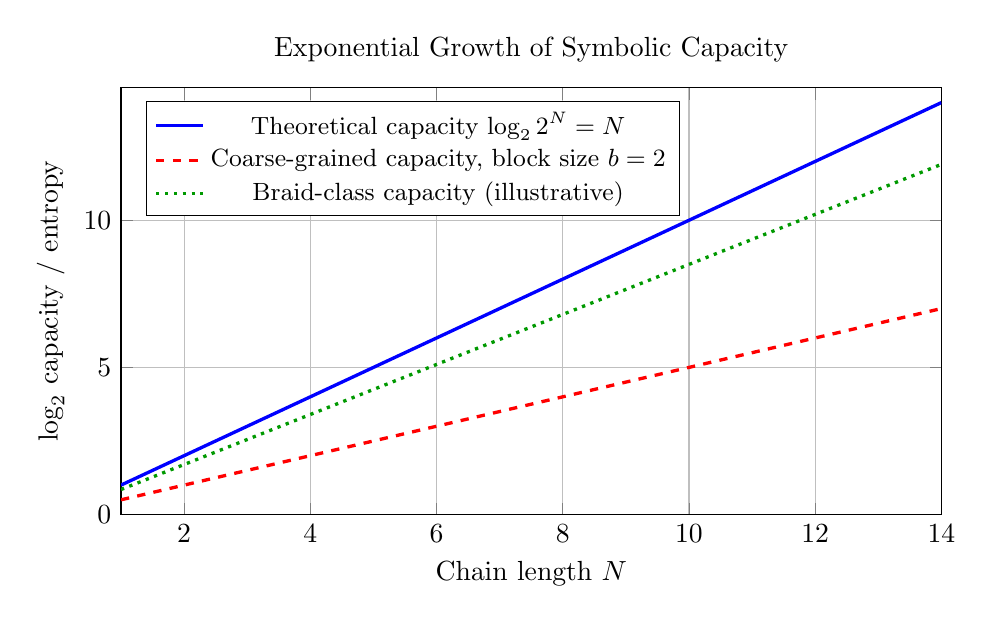
\begin{tikzpicture} \begin{axis}[ width=12cm, height=7cm, xlabel={Chain length $N$}, ylabel={$\log_2$ capacity / entropy}, xmin=1, xmax=14, ymin=0, ymax=14.5, grid=major, legend pos=north west, legend style={font=\small}, title={Exponential Growth of Symbolic Capacity} ] \addplot[domain=1:14, samples=14, blue, very thick] {x}; \addlegendentry{Theoretical capacity $\log_2 2^N = N$} \addplot[domain=1:14, samples=14, red, dashed, very thick] {0.5*x}; \addlegendentry{Coarse-grained capacity, block size $b=2$} \addplot[domain=1:14, samples=14, green!60!black, dotted, very thick] {0.85*x}; \addlegendentry{Braid-class capacity (illustrative)} \end{axis} \end{tikzpicture} \caption{\textbf{Exponential growth of symbolic capacity with chiral chain length.} A binary chiral alphabet produces $2^N$ distinct configurations for an $N$-site chain. Coarse-graining reduces but preserves exponential growth; spatial braiding further expands the distinguishable symbol set.} \label{fig:capacity} \end{figure}




\begin{figure}[htbp]
\centering
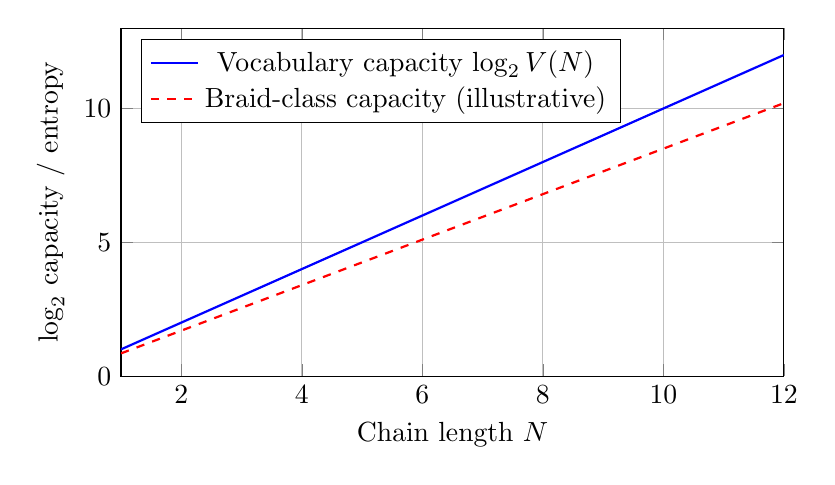
\begin{tikzpicture}
\begin{axis}[
    width=10cm, height=6cm,
    xlabel={Chain length $N$},
    ylabel={$\log_2$ capacity / entropy},
    xmin=1, xmax=12, ymin=0, ymax=13,
    grid=major,
    legend pos=north west
]
\addplot[domain=1:12, samples=12, blue, thick] {x};
\addlegendentry{Vocabulary capacity $\log_2 V(N)$}
\addplot[domain=1:12, samples=12, red, dashed, thick] {0.85*x};
\addlegendentry{Braid-class capacity (illustrative)}
\end{axis}
\end{tikzpicture}
\caption{Exponential growth of symbolic capacity with chiral chain length. The dashed line illustrates the additional capacity introduced by spatial braiding.}
\label{fig:capacity}
\end{figure}

\begin{figure}[htbp]
\centering
\begin{tikzpicture}[scale=0.9]
\node[draw, rounded rectangle, fill=blue!10, align=center] (micro) at (-4.5,0) {Fine quantum world\\$|\chi_1\rangle\otimes\cdots\otimes|\chi_N\rangle$};
\node[draw, rounded rectangle, fill=green!10, align=center] (lang) at (0,0) {Coarse-grained language\\token $w=\hat C|\Psi_f\rangle$};
\node[draw, rounded rectangle, fill=orange!10, align=center] (macro) at (4.5,0) {Macroscopic cosmos\\galaxies, universe};
\draw[->, thick] (micro) -- node[above]{$\hat C$} (lang);
\draw[->, thick] (lang) -- node[above]{describes} (macro);
\node at (-4.5,-1.2) {chirality $L/R$};
\node at (0,-1.2) {effective $L$};
\node at (4.5,-1.2) {dominant $L$};
\end{tikzpicture}
\caption{The CQL mediation scheme. Fine chiral microstates are coarse-grained into language tokens, which in turn describe macroscopic chiral structures.}
\label{fig:scheme}
\end{figure}

\section{Discussion}

The CQL hypothesis offers a unified answer to the puzzle posed in the title: language can describe both microscopic quanta and the macroscopic cosmos because it is itself a coarse-grained chiral quantum system embedded in a homochiral universe. The same operator that maps electron chirality to words also maps galaxy chirality to words, because both the microstate and the macrostate share the effective handedness of the universe.

The framework also explains---in combinatorial terms---how two chiralities can yield 64 hexagrams or a million dictionary entries. A binary alphabet, arranged in chains and braids, produces exponential diversity. This turns the author’s original intuition about divination into a concrete model of symbolic encoding.

We emphasize the speculative status of the proposal. The chirality of language is an effective, not a literal, quantum property. The divination and \emph{yuanfen} analogies are heuristic, not evidence. The predictions in Section 5 are deliberately risky: if large-scale semantic networks turn out to be parity-symmetric, or if galaxy spins show no preferred handedness, the CQL hypothesis will be correspondingly constrained. This is the proper fate of any scientific idea.

If any of the predicted correlations were confirmed, the implications would be profound. It would suggest that the structure of human language carries physical information about parity violation and cosmic homochirality---a bridge between physics, biology, and linguistics that is rarely contemplated.

\section*{Data and Code Availability}

All data used in the proposed benchmarks are publicly available: Small World of Words (SWOW) \cite{deyoe19}, ConceptNet \cite{speer17}, PubChem \cite{kim16}, and the Galaxy Zoo/SDSS catalogues \cite{lintott11}. The simulation code and any derived datasets are available at \url{https://github.com/xiaohui-li-lab/2026-11-8/}.

\section*{Author Contributions}

X.L. conceived the CQL hypothesis, designed the theoretical framework and simulations, wrote the manuscript, and prepared the code repository.

\section*{Competing Interests}

The author declares no competing interests.

\begin{thebibliography}{99}

\bibitem{wu57}
C. S. Wu, E. Ambler, R. W. Hayward, D. D. Hoppes, and R. P. Hudson,
``Experimental Test of Parity Conservation in Beta Decay,''
\textit{Phys. Rev.} \textbf{105}, 1413--1414 (1957).

\bibitem{pasteur48}
L. Pasteur,
``Recherches sur les relations qui peuvent exister entre la forme cristalline, la composition chimique et le sens de la polarisation rotatoire,''
\textit{Ann. Chim. Phys.} \textbf{24}, 442--459 (1848).

\bibitem{quack02}
M. Quack,
``Molecular Parity Violation and Chirality: The Asymmetry of Life and the Symmetry Violations in Physics,''
in \textit{Chirality in Natural and Applied Science}, pp. 125--158 (Blackwell, 2002).

\bibitem{glashow61}
S. L. Glashow,
``Partial-Symmetries of Weak Interactions,''
\textit{Nucl. Phys.} \textbf{22}, 579--588 (1961).

\bibitem{salam68}
A. Salam,
``Weak and Electromagnetic Interactions,''
in \textit{Elementary Particle Physics}, ed. N. Svartholm, pp. 367--377 (Almqvist \& Wiksell, 1968).

\bibitem{kondepudi85}
D. K. Kondepudi and G. W. Nelson,
``Weak Neutral Currents and the Origin of Biomolecular Chirality,''
\textit{Nature} \textbf{314}, 438--441 (1985).

\bibitem{cronin97}
J. R. Cronin and S. Pizzarello,
``Enantiomeric Excesses in Meteoritic Amino Acids,''
\textit{Science} \textbf{275}, 951--955 (1997).

\bibitem{longo11}
M. J. Longo,
``Evidence for a Preferred Handedness of Spiral Galaxies,''
arXiv:1101.0516 [astro-ph.CO] (2011).

\bibitem{hutsemekers05}
J. Hutsem\'ekers, H. Lamy, and D. Willaime,
``Mapping Extreme-Scale Alignments of Quasar Polarization Vectors,''
\textit{Astron. Astrophys.} \textbf{441}, 915--930 (2005).

\bibitem{wilhelm50}
R. Wilhelm and C. F. Baynes (trans.),
\textit{The I Ching or Book of Changes} (Princeton Univ. Press, 1950).

\bibitem{goldenfeld92}
N. Goldenfeld,
\textit{Lectures on Phase Transitions and the Renormalization Group} (Addison-Wesley, 1992).

\bibitem{gardenfors00}
P. G\"ardenfors,
\textit{Conceptual Spaces: The Geometry of Thought} (MIT Press, 2000).

\bibitem{mermin79}
N. D. Mermin,
``The topological theory of defects in ordered media,''
\textit{Rev. Mod. Phys.} \textbf{51}, 591--648 (1979).

\bibitem{read99}
N. Read and D. Green,
``Paired states of fermions in two dimensions with breaking of parity and time-reversal symmetries,''
\textit{Phys. Rev. B} \textbf{61}, 10267--10297 (2000).

\bibitem{aubin98}
T. Aubin and P. Jouventin,
``Cocktail-party effect in king penguin colonies,''
\textit{Proc. R. Soc. Lond. B} \textbf{265}, 1665--1673 (1998).

\bibitem{deyoe19}
M. De Deyne et al.,
``The Small World of Words: English word association norms for over 12,000 cue words,''
\textit{Behav. Res. Methods} \textbf{51}, 987--1006 (2019).

\bibitem{speer17}
R. Speer, J. Chin, and C. Havas,
``ConceptNet 5.5: An Open Multilingual Graph of General Knowledge,''
in \textit{Proc. AAAI} (2017).

\bibitem{kim16}
S. Kim et al.,
``PubChem Substance and Compound databases,''
\textit{Nucleic Acids Res.} \textbf{44}, D1202--D1213 (2016).

\bibitem{lintott11}
C. Lintott et al.,
``Galaxy Zoo 1: data release of morphological classifications for nearly 900,000 galaxies,''
\textit{Mon. Not. R. Astron. Soc.} \textbf{410}, 166--178 (2011).

\bibitem{hegstrom80}
R. A. Hegstrom, D. W. Rein, and P. G. H. Sandars,
``Calculation of the parity nonconserving energy difference between mirror-image molecules,''
\textit{J. Chem. Phys.} \textbf{73}, 2329--2341 (1980).

\end{thebibliography}
\textbf{\textbf{Declarations}}

  
  
  \textbf{\textbf{Acknowledgements}}

The author thanks colleagues for discussions on quantum aggregates, consciousness, emergence, and dimensionality. 

 \textbf{\textbf{Funding Statement}}:This research did not receive any specific grant from funding agencies in the public,commercial,or not-for-profit sectors.

Currently, there are no sponsors. Or I haven't found any sponsors or organizations yet. However, if I can publish it, I will cover part of the costs myself. Or it will be easier to find sponsors. (For example, the German company E.ON. I have previously found international buyers for their wind turbines.)

 \textbf{\textbf{Competing Interests}}

The author declares no competing interests.

 \textbf{\textbf{Author Contributions}}

Xiaohui Li: Conceptualization, Methodology, Investigation, Formal analysis, Writing – Original Draft, Visualization, Writing – Review \& Editing.

AI assisted me in rewriting the original text into an article that meets the submission requirements of Journal of the American Mathematical Society. No content was added or omitted.

 The author is solely responsible for the work described in this manuscript and has approved the final version for publication.

 \textbf{\textbf{Clinical trial:}}not applicable.

 \textbf{\textbf{Ethics and Consent to Participate declarations}}: not applicable.

 Hi,

This is an original work by the author. There is only one author:Xiaohui Li.

The article accurately reflects the scientific results.

Xiaohui Li agreed to submit the manuscript.

This manuscript has not been published in any other journals.

The author accepts the established procedure for selecting and publishing manuscripts.

good

Xiaohui Li



 \textbf{\textbf{Clinical trial number}}: not applicable.
 
 \textbf{\textbf{Declaration of Competing Interests}}: 

The authors declare that they have no competing interests.
\end{document}
